\chapter{Vibrations of a viscoelastic bar}
\label{chapter:viscoelastic-bar-vibrations}

Consider the elastic bar shown in figure~\ref{fig:viscoelastic-bar}. It is fixed on the left hand side and free on the right, has a length of $L$ and can undergo longitudinal motion as described by the function $u(x,\,t)$. We want to calculate its (undamped) natural frequencies $\omega_0$ and associated damping ratios $\zeta$.

\begin{figure}[h]
\centering
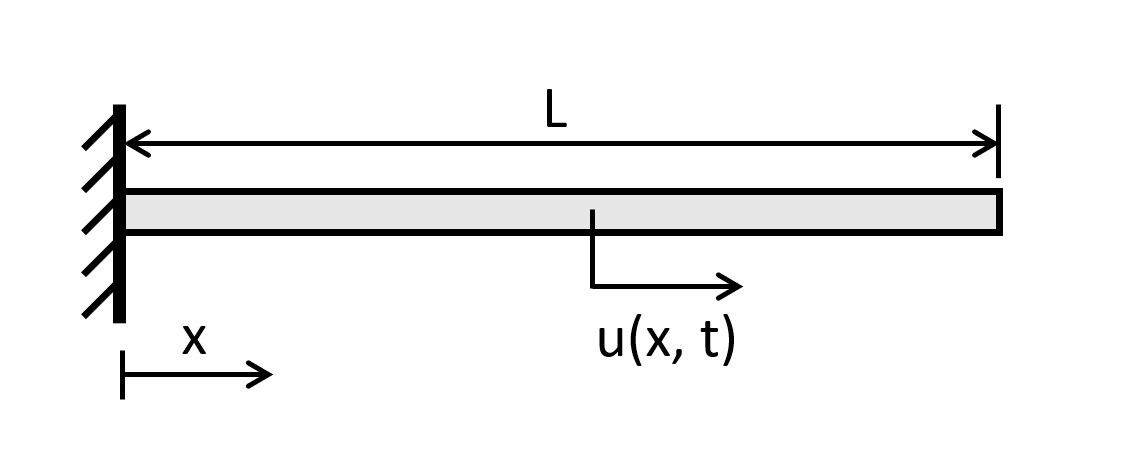
\includegraphics[width=0.5\textwidth]{figures/appendix/viscoelastic-bar}
\caption{Kinematics and boundary conditions of the bar}
\label{fig:viscoelastic-bar}
\end{figure}

The material of the bar is assumed to behave according to the viscoelastic Kelvin-Voigt model, which expresses the stress $\sigma$ in the bar as
%
\begin{equation}
\sigma = E\,\varepsilon + \eta\,\dot{\varepsilon}\label{eq:viscoelastic-bar-material}
\end{equation}

where $\varepsilon = \frac{\partial\,u}{\partial\,x}$ is the longitudinal strain, $E$ the elastic modulus and $\eta$ the viscosity of the material. The acceleration at every point in the bar is given by \textcolor{red}{Source?}
%
\begin{equation}
\rho\,\frac{\partial^2\,u}{\partial\,t^2} = \frac{\partial\,\sigma}{\partial\,x}\label{eq:viscoelastic-bar-kinetic}
\end{equation}

where $\rho$ is the bar's density. Combining the equations (\ref{eq:viscoelastic-bar-material}) and (\ref{eq:viscoelastic-bar-kinetic}) and multiplying with the cross section area $A$ results in the equation of motion
%
\begin{equation}
\rho A\,\frac{\partial^2\,u}{\partial\,t^2} = EA\,\frac{\partial^2\,u}{\partial\,x^2} + \eta A\,\frac{\partial^3\,u}{\partial\,x^2\,\partial\,t}.\label{eq:viscoelastic-bar-motion}
\end{equation}

This partial differential equation can be solved by separation of variables. The solution is assumed as $u(x,\,t) = X(x)\,T(t)$, a product of two functions depending on $x$ and $t$ respectively. Inserting this into the equation of motion (\ref{eq:viscoelastic-bar-motion}) and separating terms depending on $x$ from terms depending on $t$ leads to
%
\begin{align}
\rho A\,X(x)\,\ddot{T}(t) &= EA\,X''(x)\,T(t) + \eta A\,X''(x)\,\dot{T}(t)\notag \\
\frac{X''(x)}{X(x)} &= \frac{\ddot{T}(t)}{\frac{EA}{\rho A}\,T(t) + \frac{\eta A}{\rho A}\,\dot{T}(t)} =: -\frac{\rho A}{EA}\,\omega_0^2\label{eq:viscoelastic-bar-separated}
\end{align}

Apply the usual argument: As one side of the equation depends on position and the other on time they have to be constant in order to be equal. We choose that constant to be $-\frac{\rho A}{EA}\,\omega_0^2$ and obtain the two ordinary differential equations
%
\begin{align}
\ddot{T}(t) + \frac{\eta A}{EA}\,\omega_0^2\,\dot{T}(t) + \omega_0^2\,T(t) = 0,\label{eq:viscoelastic-bar-t} \\
X''(x) + \frac{\rho A}{EA}\,\omega_0^2\,X(x) = 0.\label{eq:viscoelastic-bar-x}
\end{align}

The time equation (\ref{eq:viscoelastic-bar-t}) describes a damped harmonic oscillator with undamped natural frequency $\omega_0$ and damping ratio
%
\begin{equation}
\zeta = \frac{1}{2}\,\frac{\eta\,A}{EA}\,\omega_0\label{eq:viscoelastic-bar-result-zeta}
\end{equation}

as determined by the coefficients of the equation. The last remaining task is to determine the natural frequencies $\omega_0$ which solve the second differential equation (\ref{eq:viscoelastic-bar-x}) while also satisfying the boundary conditions of the bar. The general solution of (\ref{eq:viscoelastic-bar-x}) is
%
\begin{equation}
X(x) = C\cdot\sin\left(\sqrt{\frac{\rho A}{EA}}\,\omega_0\,x - \varphi\right).
\end{equation}

Boundary condition on the fixed end:
%
\begin{align}
u(0,\,t) = 0: \quad\quad\quad X(0)\,T(t) &= 0 \notag \\
C\cdot\sin(-\varphi) &= 0 \notag \\
\varphi &= 0
\end{align}

The case $T(t) = 0$ was ignored here because it is of no interest. The boundary condition for the free end is
%
\begin{align}
\sigma(L,\,t) = 0: \quad\quad E\,\varepsilon(L,\,t) + \eta\,\dot{\varepsilon}(L,\,t) &= 0 \notag \\
EA\,\frac{\partial u}{\partial x}(L,\,t) + \eta A\,\frac{\partial^2 u}{\partial x\,\partial t}(L,\,t) &= 0 \notag \\
EA\,X'(L)\,T(t) + \eta A\,X'(L)\,\dot{T}(t) &= 0 \notag \\
(EA\,T(t) + \eta A\,\dot{T}(t))\,X'(L) &= 0 \notag \\
\ddot{T}(t)\,X'(L) &= 0 \notag
\end{align}

And therefore the solution for the natural frequencies is
%
\begin{align}
X'(L) &= C\cdot\sqrt{\frac{\rho A}{EA}}\,\omega_0\cos\left(\sqrt{\frac{\rho A}{EA}}\,\omega_0\,L\right) = 0, \notag \\
\omega_0 &= \frac{\pi(2k - 1)}{2L}\cdot\sqrt{\frac{EA}{\rho A}},\quad k \in \mathbb{Z}.\label{eq:viscoelastic-bar-result-omega}
\end{align}

And finally, with equations (\ref{eq:viscoelastic-bar-result-zeta}) and (\ref{eq:viscoelastic-bar-result-omega}) the damping ratio follow as
%
\begin{equation}
\zeta = \frac{\pi(2k - 1)}{4L}\cdot\frac{\eta A}{\sqrt{\rho A \cdot EA}},\quad k \in \mathbb{Z}.
\end{equation}